\documentclass{report}
\usepackage[utf8]{inputenc}
\usepackage{enumitem}
\usepackage{graphicx}
\usepackage{hyperref}

\hypersetup{
    colorlinks=true,
    linkcolor=blue,
    filecolor=magenta,      
    urlcolor=cyan,
    pdfpagemode=FullScreen,
}
\urlstyle{same}

\graphicspath{ {./images} }

%%% FORMATTING %%%
\usepackage{geometry}
\geometry{
    a4paper,
    left=25mm,
    right=25mm,
    top=10mm,
    bottom=20mm,
}

\newcommand{\code}[1]{\texttt{#1}}

\begin{document}

\chapter*{Chapter 1 exercises}
This document contains the solutions for the exercises going through the prolog primer to prepare for AI.
\section*{\textbf{Exercise 1.1}}
\begin{enumerate}[label=(\alph*)]
    \item \emph{Which of the following are valid Prolog atoms?}
    
    This was verified in SWI-Prolog using \code{atom()}
    \begin{itemize}[label={}]
        \item \code{f}: Valid 
        \item \code{loves(john, mary)}: Invalid, this is a compound term
        \item \code{Mary}: Invalid, this is a variable
        \item \code{\_c1}: Invalid, this is a variable
        \item \code{'Hello'}: Valid, you can use single quotes to make any string an atom
        \item \code{this\_is\_it}: Valid
    \end{itemize}

    \item \emph{Which of the following are valid names for Prolog vairables?}
    
    This was verified in SWI-Prolog using \code{var()}
    \begin{itemize}[label={}]
        \item \code{a}: Invalid, must start with uppercase or underscore
        \item \code{A}: Valid
        \item \code{Paul}: Valid
        \item \code{'Hello'}: Invalid, single quotes denote atoms
        \item \code{a\_123}: Invalid
        \item \code{\_ }: Valid, anonymous variable
        \item \code{\_abc}: Valid
        \item \code{x2}: Valid
    \end{itemize}

    \item \emph{What would a Prolog interpreter reply given the following query?}

    \centerline{\code{?- f(a, b) = f(X, Y).}}
    
    The interpreter would instantiate X = a and Y = b, as this will evaluate the query to be true: \\
    \code{X = a} \\
    \code{Y = b} \\
    \code{true} \\

    \item \emph{Would the following query succeed?}
    
    \centerline{\code{?- loves(mary, john) = loves(John, Mary).}}

    This query would suceed. Both John and Mary are variables, so the interpreter would instantiate John = john and Mary = mary, causing the statements to match.

    \item \emph{Assume a program consisting only of the fact }  \code{a(B, B).} \emph{has been consulted by Prolog. How will the system react to the following query?}
    
    \centerline{\code{?- a(1, X), a(X, Y), a(Y, Z), a(Z, 100).}}

    Prolog will return \textbf{false}. The first query causes X = 1, the subsequent query causes Y = 1, then Z = 1, and the final query will fail as 1 and 100 are different.

\end{enumerate}

\section*{\textbf{Exercise 1.2}}
Understand and explain the following queries:
\begin{enumerate}[label=(\alph*)]

    \item \code{?- myFunctor(1, 2) = X, X = myFunctor(Y, Y).}
    
    The interpreter will instantiate X = myFunctor(1, 2) to match the first clause. On the following clause, the equality fails, as the numbers inside the compound term X are not the same. As Y cannot be instantiated to both 1 and 2, the query is \textbf{false}.

    \item \code{?- f(a, \_, c, d) = f(a, X, Y, \_).}
    
    The interpreter will match the \_ on the left-hand side to X. It will then instaniate Y = c, and the \_ on the right-hand side to d. The query will return \textbf{true}. An interesting thing to note from running the query is that only the Y = c instantiation is displayed, as the \_ variables are ignorable.

    \item \code{?- write('One '), X = write('Two ').}
    
    The \code{write()} predicate always returns true (as well as writing text in the command line). This means the first clause passes, and the string literal "One " is printed. For the second clause, the variable X is initialised as X = write('Two '), meaning the interpreter instead views write() as a compound term that it can assign to X. This makes the equality pass and so the overall query returns \textbf{true}.

\end{enumerate}

\section*{\textbf{Exercise 1.3}}
\emph{Draw the family tree corresponding to the following Prolog program:}

\noindent\emph{N.B. I couldn't be bothered writing out everything, for reference see Exercise 1.3 of \href{run:./PrologPrimer.pdf}{PrologPrimer.pdf}}

\begin{figure}[h]
    \centering
    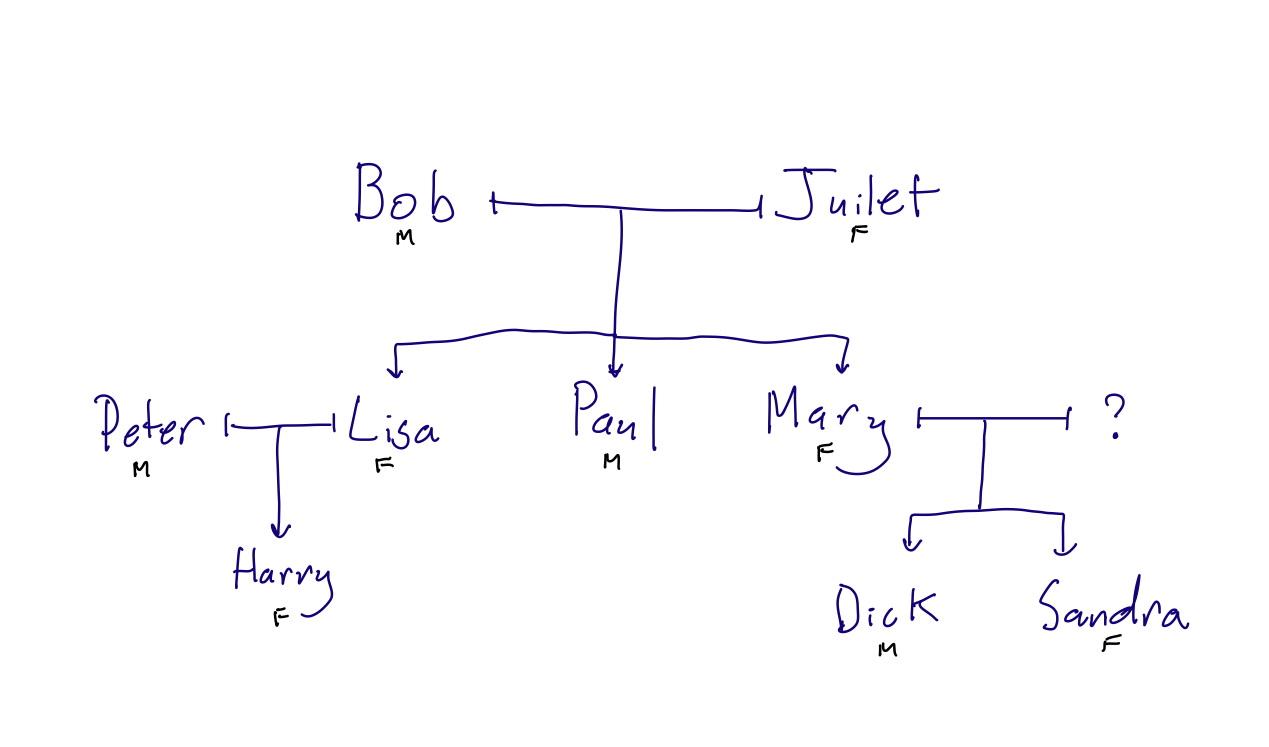
\includegraphics[width=1\textwidth]{Family_Tree.png}
    \label{fig:Family_Tree}
\end{figure}

\noindent\emph{Define ne predicates (in terms of rules using male/1, female/1 and parent/2) for the following family relations: (/x denotes the number of 'arguments')}

\begin{enumerate}[label=(\alph*)]
    \item \code{father(X, Y) :- parent(X, Y), male(X)}
    \item \code{sister(X, Y) :- parent(A, X), parent(A, Y), parent(B, X), parent(B, Y), female(X)}
    \item \code{grandmother(X, Y) :- parent(Z, Y), parent(X, Z), female(X)}
    \item \code{cousin(X, Y) :- grandparent(Z, X), grandparent(Z, Y), notsibling(X, Y)}
    
    \code{grandparent(X, Y) :- parent(Z, Y), parent(X, Z)}

    \code{notsibling(X, Y) :- parent(A, X), parent(B, X), \textbackslash+ parent(A, Y), \textbackslash+ parent(B, Y)}
    

\end{enumerate}



\end{document}